% modify sensitivity parameter in unobserved likelihood
% Time-stamp: <liuminzhao 07/14/2014 21:34:40>

\documentclass[12pt]{article}

\usepackage[figuresright]{rotating}
\usepackage{amsmath}
\usepackage{bm}
\usepackage{color}

\usepackage{amsmath}
\usepackage[round]{natbib}
%\usepackage{times}
\usepackage{graphicx}
%\usepackage{courier}
\usepackage{mathpazo}
\usepackage{mathrsfs}
\usepackage{bm}
\usepackage[colorlinks,linkcolor=red,anchorcolor=blue,citecolor=blue]{hyperref}
\usepackage[verbose,letterpaper,tmargin=1in,bmargin=.75in,lmargin=.75in,rmargin=1in]{geometry}
\usepackage{amsthm}
\usepackage{pdflscape}
\usepackage{authblk}

\newtheorem{thm}{Theorem}[section] \newtheorem{deff}[thm]{Definition}
\newtheorem{rmk}[thm]{Remark} \newtheorem{prf}[thm]{Proof}
\newtheorem{cor}[thm]{Corollary} \newtheorem{emp}[thm]{Example}
\newtheorem{lem}[thm]{Lemma} \newtheorem{pps}[thm]{Proposition}
\newcommand{\iid}{\stackrel{\mbox{i.i.d}}{\sim}}
\newcommand{\pr}{\mbox{p}}
\newcommand{\prob}{\mbox{Pr}}
\newcommand{\polya}{P\'{o}lya} \newcommand{\yobs}{\bm y_{\it{obs}}}
\newcommand{\ymis}{\bm y_{\it{mis}}}


%%%%%%%%%%%%%%%%%%%%%%%%%%%%%%

\title{Quantile Regression in the Presence of Monotone Missingness with Sensitivity Analysis}

\author[1]{Minzhao Liu\thanks{liuminzhao@ufl.edu}}
\author[2]{Michael J. Daniels\thanks{mjdaniels@austin.utexas.edu}}
\author[3]{Michael G. Perri\thanks{mperri@phhp.ufl.edu}}
\affil[1]{Department of Statistics, University of Florida, FL 32601, USA}
\affil[2]{Department of Integrative Biology, Division of Statistics and Scientific Computation\\
The University of Texas at Austin, 141MC Patterson Hall, Austin, TX 78712, USA}
\affil[3]{Department of Clinical and Health Psychology, University of Florida, Gainesville, FL 32611, USA}

\usepackage{setspace}
\linespread{2}

\providecommand{\keywords}[1]{\textbf{\textit{Index terms---}} #1}

\begin{document}

\maketitle{}

\begin{abstract}
  In this paper, we develop methods for longitudinal quantile regression when there is monotone missingness.
  In particular, we propose pattern mixture models with a constraint that provides a straightforward interpretation of the marginal quantile regression parameters.
  Our approach allows sensitivity analysis which is an essential component in inference for incomplete data.
  To facilitate computation of the likelihood, we propose a novel way to obtain analytic forms for the required integrals.  We conduct simulations to examine the robustness of our approach to modeling assumptions and compare its performance to competing approaches.
  The model is applied to data from a recent clinical trial on weight management.

{\bf keywords:} Marginalized models, Non-ignorable missingness, Pattern mixture models.
\end{abstract}



\section{Introduction}

Quantile regression is used to study the relationship between a
response and covariates when one (or several) quantiles are of
interest as opposed to mean regression.  The dependence between upper
or lower quantiles of the response variable and the covariates often
vary differentially relative to that of the mean. How quantiles depend
on covariates is of interest in econometrics, educational studies,
biomedical studies, and environment studies \citep{yu2001,
  buchinsky1994,buchinsky1998,he1998, koenker1999,wei2006,yu2003}. A
comprehensive review of applications of quantile regression was
presented in \citet{koenker2005}.

Quantile regression is more robust to outliers than mean regression
and provides information about how covariates affect quantiles, which
offers a more complete description of the conditional distribution of
the response. Different effects of covariates can be assumed for
different quantiles.

The traditional frequentist approach was proposed by
\citet{koenker1978} for a single quantile with estimators derived by
minimizing a loss function. The popularity of this approach is due to
its computational efficiency, well-developed asymptotic properties,
and straightforward extensions to simultaneous quantile regression and
random effect models. However, the approach does not naturally
extend to missing data.
Extensions of minimizing loss function include the use of regularization.
\citet{koenker2004} adopted $l_1$ regularization methods to shrink a large number of individual effects to a common value for quantile regression models for longitudinal data.
\citet{li2008} considered $L_1$-norm (LASSO) regularized quantile regression.
\citet{wu2009} demonstrated using a smoothly clipped absolute deviation model for variable selection in penalized quantile regression.
In terms of Bayesian inference, both parametric and semiparametric Bayesian approaches have been proposed in the literature \citep{yu2001,walker1999,hanson2002,reich2010}.

All the above methods focus on complete data.  There are only a few
articles about quantile regression with missingness.  \citet{wei2012}
proposed a multiple imputation method for quantile regression model
when there are some covariates missing at random (MAR). They impute
the missing covariates by specifying its conditional density given
observed covariates and outcomes, which come from the estimated
conditional quantile regression and specification of conditional
density of missing covariates given observed ones.
However, they focus more on the missing covariates than missing outcomes.
\citet{bottai2013} introduced an imputation method using estimated
conditional quantiles of missing outcomes given observed data. Their
approach does not make distributional assumptions.  They assumed the
missing data mechanism (MDM) is MAR. However, because their
imputation method is not derived from a joint distribution, the joint
distribution under such conditionals may not exist.  In addition, their
approach does not allow for missing not at random (MNAR).

\citet{yuan2010} introduced a fully parametric Bayesian quantile
regression approach for longitudinal data with non-ignorable missing
data. They used shared latent subject-specific random effects to
explain the within-subject correlation and to associate the response
process with missing data process, and applied multivariate normal
priors on the random terms to match the traditional quantile
regression check function with penalties. However, the quantile
regression coefficients are conditional on the random effects, which
is not of interest if we are interested in interpreting regression
coefficients unconditionally.  In addition, they are
conditional on random effects, which tie together the responses and
missingness process, so they have a slightly different interpretation
than typical random effects in longitudinal methods. Moreover, due to
their full parametric specification for the full data, their model
does not allow for sensitivity analysis, which is a key component in
inference for incomplete data \citep{nas2010}.

Pattern mixture models were originally proposed to model missing data
in \citet{rubin1977}. Later mixture models were extended to handle
MNAR in longitudinal data. For discrete dropout times,
\citet{little1993, little1994} proposed a general method by
introducing a finite mixture of multivariate distribution for
longitudinal data. When there are many possible dropout time,
\citet{roy2003} proposed to group them by latent classes.

\citet{roy2008} extended \citet{roy2003} to generalized linear models
and proposed a pattern mixture model for data with non-ignorable
dropout, borrowing ideas from \citet{heagerty1999}.  But their
approach only estimates the marginal covariate effects on the mean. We
will use related ideas for quantile regression models which allow for
non-ignorable missingness and sensitivity analysis.

The structure of this article is as follows. First, we introduce a
quantile regression method to address monotone non-ignorable
missingness in section \ref{ch3:sec:model}, including sensitivity analysis
and computational details.  We use simulation studies to evaluate the
performance of the model in section \ref{ch3:sec:simulation}. We apply our
approach to data from a recent clinical trial in section
\ref{ch3:sec:real}. Finally, discussion and conclusions are given in
section \ref{ch3:sec:discussion}.

\section{Model}
\label{ch3:sec:model}

In this section, we first introduce some notation, then describe our proposed quantile regression model in section \ref{ch3:sec:settings}.
We provide details on MAR and MNAR and computation in sections \ref{ch3:sec:sa} and \ref{ch3:sec:computation} respectively.

Under monotone dropout, denote $S_i \in \{1, 2, \ldots, J\}$ to be the number of observed $Y_{ij}^{\prime} s$ for subject $i$,
and $\bm Y_i = (Y_{i1}, Y_{i2}, \ldots, Y_{iJ})^{T}$ to be the full data response vector for subject $i$, where $J$ is the maximum follow up time.
We assume $Y_{i1}$ is always observed.
We are interested in the $\tau$-th marginal quantile regression coefficients $\bm \gamma_j = (\gamma_{j1}, \gamma_{j2}, \ldots, \gamma_{jp})^T$,
\begin{equation}\label{eq:marg}
  \prob (Y_{ij} \leq \bm x_i^{T} \bm \gamma_j ) = \tau, \mbox{ for } j = 1, \ldots, J,
\end{equation}
where $\bm x_i$ is a $p \times 1$ vector of covariates for subject
$i$.

Let
\begin{displaymath}
  \pr_k(Y) = \pr (Y | S = k), \quad  \pr_{\geq k} (Y)  = \pr (Y | S \geq k)
\end{displaymath}
be the densities of response $\bm Y$ given $S=k$ and $S
\geq k$. And $\prob_k$ be the corresponding probability given $S = k$.

\subsection{Mixture Model Specification}
\label{ch3:sec:settings}
We adopt a pattern mixture model to jointly model the response and missingness \citep{little1994, dh2008}.
Mixture models factor the joint distribution of response and missingness as
\begin{displaymath}
  \pr (\bm y, \bm S, |\bm x, \bm \omega) = \pr (\bm y|\bm S, \bm x, \bm \omega) \pr (\bm S | \bm x, \bm \omega).
\end{displaymath}
Thus the full-data response follows the distribution given by
\begin{displaymath}
  \pr (\bm y | \bm x, \bm \omega) = \sum_{S \in \mathcal{S}} \pr(\bm y| \bm S, \bm x, \bm \theta) \pr (\bm S | \bm x, \bm \phi),
\end{displaymath}
where $\mathcal{S}$ is the sample space for the number of observed responses, $S$ (i.e., the pattern) and the parameter vector $\bm \omega$ is partitioned as $(\bm \theta, \bm \phi)$.

Furthermore, the conditional distribution of response within patterns can be decomposed as
\begin{equation}\label{eq:decompose}
  \pr (\yobs, \ymis | \bm S, \bm \theta) = \pr
  (\ymis|\yobs, \bm S, \bm \theta_E) \pr (\yobs | \bm S, \bm
  \theta_{y, O}),
\end{equation}
where $\bm \theta_E$ indexes the parameters in the extrapolation distribution,
the first term on the right hand side and $\bm \theta_{y, O}$ indexes parameters in the distribution of observed responses, the second term on the right hand side.
As in \cite{dh2008}, we denote $\bm \xi(\bm \omega) = (\bm \xi_m, \bm \xi_s)$ as a possible reparametrization of the parameters in the full data model above where $\bm \xi_s$ are sensitivity parameters (not identified by the observed data) and $\bm \xi_m$ are identified by the observed data (just the parameters of the observed data distribution).

We assume a sequential finite ($K$) mixture of normals within each pattern.
A random variable $x$ follows a finite ($K$) mixture of normal distribution (MN), when
\begin{displaymath}
p(x|\bm \theta) = \sum_{i = 1}^K \omega_i \phi_N(x; \mu_i, \sigma_i^2),
\end{displaymath}
where $\bm \theta = (\bm{\mu, \sigma^2, \omega})$, $\bm \mu = (\mu_1, \ldots, \mu_K), \bm \sigma = (\sigma_1, \ldots, \sigma_K), \bm \omega = (\omega_1, \ldots, \omega_K)$,
and $\phi_N(x; \mu, \sigma^2)$ denotes the PDF evaluated at $x$ of a normal distribution with mean $\mu$ and variance $\sigma^2$.

In particular, we specify the distributions conditional on $S=k$ as:
\begin{equation}
  \begin{array}{l}
      \displaystyle Y_{i1} = \Delta_{i1} +  \bm{x_{i}^T\beta_1^{(k)}} + \epsilon_{i1} , k = 1, \ldots, J,\\
       \displaystyle        Y_{ij}|\bm Y_{ij^{-}} =
      \begin{cases}
        \Delta_{ij} + \bm y_{ij^{-}}^T \bm \beta_{y,j-1} + \epsilon_{ij}, & k \geq j ;  \\
        \chi(\bm x_{i}, \bm y_{ij^{-}}) + \epsilon_{ij}, & k < j ;  \\
      \end{cases}, \mbox{ for } 2 \leq j \leq J,  \\
       S_{i} = k \sim \textrm{Multinomial}(1, \bm \phi),
    \end{array}
  \label{eq:model}
\end{equation}
where
\begin{equation}
\begin{aligned}
\epsilon_{ij} |\bm \theta & \iid \mbox{MN}(\bm \theta),  \\
\bm \theta & = (\mu_l, \sigma_l, \omega_l), l = 1, \ldots, K,
\end{aligned}\label{eq:mixprob}
\end{equation}
with the marginal quantile regression constraints \eqref{eq:marg}.
The parameter $\bm \beta_1^{(k)}$ is the shift of the coefficients for distribution of $Y_{i1} | S = k$,
$\bm y_{ij^{-}} = (y_{i1}, \ldots, y_{i(j-1)})^T$ is the response history for subject $i$ up to time point  $(j-1)$,
$\bm \beta_{y, j-1} = \big(\beta_{y_1, j-1}, \ldots, \beta_{y_{j-1}, j-1} \big)^T$ are autoregressive coefficients,
$\sigma_j$ is the conditional standard deviation of response component $j$, and
$\bm \phi = (\phi_1, \ldots, \phi_J)$ is the multinomial probability vector for the number of observed responses.
$\Delta_{ij}$ are subject/time specific intercepts determined by the parameters in (\ref{eq:marg}) and (\ref{eq:model}); more details are given in what follows.
$\chi(\bm x_{i}, \bm y_{ij^{-}})$ is the mean of the unobserved data distribution and allows sensitivity analysis by varying assumptions on $\chi$; for computational reasons we assume that $\chi$ is linear in $y_{ij^{-}}$.
For example, here we specify
\begin{equation}
\label{eq:model2}
\chi(\bm x_{i}, \bm y_{ij^{-}}) = \Delta_{ij}  + \bm y_{ij^{-}}^T \bm \beta_{y,j-1} + \bm{x_{i}^{T} h^{(k)}} ,
\end{equation}
where $\bm h^{(k)}$ is a set of sensitivity parameters and $\Delta_{ij}$ depends on $x_i$.
Comparing (\ref{eq:model}) and (\ref{eq:model2}), the mean of the unidentified distribution,
$\pr_k(y_{ij}|\bm y_{ij^{-}})$ for $k < j$ is characterized by an intercept shift from identified observed data distribution, $\pr_k(y_{ij}|\bm y_{ij^{-}})$ for $k \geq j$.
More details about sensitivity parameters are given in section~\ref{ch3:sec:sa}.

For (standard) identifiability of the distribution of the observed data, we use the
following restrictions (without loss of generality),
\begin{displaymath}
 \sum_{k=1}^J \beta_{1l}^{(k)} = 0.
\end{displaymath}
Also in order to not confound the marginal quantile regression parameters,
we put the following constraint on the parameters $\bm \theta$ in the mixture of normals distribution,
\begin{displaymath}
\sum_{l= 1}^K \omega_{l}\mu_{l} = 0.
\end{displaymath}

In (\ref{eq:model}) and (\ref{eq:model2}), $\Delta_{ij}$ are functions of $(\tau, \bm x_{i},
\bm \beta, \bm h, \bm \theta, \bm \gamma_j, \bm \phi)$ and are determined by the marginal
quantile regressions,
\begin{equation}
  \label{eq:deltaeqn1}
  \tau = \prob (Y_{ij} \leq \bm x_{i}^T \bm \gamma_j ) = \sum_{k=1}^J
  \phi_k\prob_k (Y_{ij} \leq \bm x_{i}^T \bm \gamma_j ) \mbox{  for  } j = 1,
\end{equation}
and
\begin{align}\label{eq:deltaeqn2}
  \tau &= \prob (Y_{ij} \leq \bm x_{i}^{T} \bm \gamma_j ) =
  \sum_{k=1}^J
  \phi_k\prob_k (Y_{ij} \leq \bm x_{i}^{T} \bm \gamma_j ) \\
  & = \sum_{k=1}^J \phi_k \int\cdots \int \prob_k (Y_{ij} \leq \bm
  x_{i}^{T} \bm \gamma_j | \bm y_{ij^{-}}
  ) \pr_k (y_{i(j-1)}| \bm y_{i(j-1)^{-}})  \nonumber \\
  & \quad \cdots \pr_k (y_{i2}| y_{i1}) \pr_k(y_{i1})
  dy_{i(j-1)}\cdots dy_{i1}.  \mbox{  for  } j = 2, \ldots, J .\nonumber
\end{align}
Details on computing the $\Delta_{ij}$ will be given in section
\ref{ch3:sec:computation}.

The idea in the above specification is to model the marginal quantile regressions directly and then to embed them in the likelihood through restrictions in the mixture model.
The finite mixture of normals distribution makes model flexible and accommodates heavy tails, skewness, and multi-modality.
The mixture model in (\ref{eq:model}) allows the marginal quantile regression coefficients to differ by quantiles; otherwise, the quantile lines would be parallel to each other.
Moreover, the mixture model also allows sensitivity analysis for the missing data.
This is an essential component of the analysis of missing data (as discussed in the introduction) and is not possible in previous approaches.

\subsection{Missing Data Mechanism and Sensitivity Analysis}
\label{ch3:sec:sa}

Mixture models as specified in Section 2.1 are not identified
by the observed data (as stated in the previous subsection). Specific forms of missingness
induce constraints to identify the distributions for
incomplete patterns, in particular, the extrapolation distribution in
(\ref{eq:decompose}). In this section, we explore ways to embed the
missingness mechanism and sensitivity parameters in mixture models for
our setting.

In the mixture model in (\ref{eq:model}), MAR holds \citep{molen1998,
  wang2011} if and only if, for each $j \geq 2$ and $k < j$:
\begin{displaymath}
  \pr_k(y_j|y_1, \ldots, y_{j-1}) = \pr_{\geq j}(y_j|y_1, \ldots, y_{j-1}).
\end{displaymath}
When $2 \leq j \leq J$ and $k < j$, $Y_j$ is not observed, thus
$(\bm{h^{(1)},\ldots,h^{(J-1)}})$ can not be identified from the
observed data.
Then $\bm \xi_s = (\bm h^{(k)}: k=1,\ldots,J-1)$ is a set
of sensitivity parameters \citep{dh2008} as mentioned earlier.

When $\bm \xi_s = \bm \xi_{s0} = \bm 0$, MAR holds. If
$\bm \xi_s$ is fixed at $\bm \xi_s \neq \bm \xi_{s0}$, the
missingness mechanism is MNAR. We can vary $\bm \xi_s$ around
$\bm 0$ to examine the impact of different MNAR mechanisms.

In general, each pattern $S = k$ has its own set of sensitivity
parameters $\bm h^{(k)}$. However, to keep the number of
sensitivity parameters at a manageable level \citep{dh2008} and
without loss of generality in what follows, we assume $\bm h^{(k)}$ does not depend
on pattern.

\subsection{Computation}
\label{ch3:sec:computation}

In section \ref{ch3:sec:deltacal}, we provide details on calculating
$\Delta_{ij}$ in (\ref{eq:model}) for $j = 1, \ldots, J$. Then we show
how to obtain maximum likelihood estimates in section
\ref{ch3:sec:mle}.

\subsubsection{Calculation of $\Delta$ }
\label{ch3:sec:deltacal}
From equation (\ref{eq:deltaeqn1}) and (\ref{eq:deltaeqn2}),
$\Delta_{ij}$ depends on subject-specific covariates $\bm x_{i}$,
thus $\Delta_{ij}$ needs to be calculated for each subject. We now
illustrate how to calculate $\Delta_{ij}$ given all the other
parameters $\bm \xi = (\bm \xi_m, \bm \xi_s)$.

\begin{itemize}
\item \textbf{$\Delta_{i1}: $} Expand equation (\ref{eq:deltaeqn1}) with (\ref{eq:model}) and (\ref{eq:mixprob}):
  \begin{align*}
    \tau = \sum_{k = 1}^J \phi_k \left( \sum_{l = 1}^{K} \omega_{l} \Phi \left( \frac{\bm x_{i}^T
        \bm \gamma_1 - \Delta_{i1} -\bm{x_i^T \beta_1^{(k)}} - \mu_{l}}{ \sigma_{l} } \right) \right).
  \end{align*}
  where $\Phi$ is the standard normal CDF.
  Because the RHS of the above equation
  is continuous and monotone in $\Delta_{i1}$, it can be solved by a
  standard numerical root-finding method (e.g. bisection method) with
  minimal difficulty.

\item \textbf{$\Delta_{ij}, 2\leq j \leq J: $}

  First we introduce a lemma:
  \begin{lem}\label{ch3:sec:lemma}
    An integral of a normal CDF with mean $b$ and standard deviation
    $a$ over another normal distribution with mean $\mu$ and standard
    deviation $\sigma$ can be simplified to a closed form in terms of
    normal CDF:
    \begin{displaymath}
      \int \Phi \left( \frac{x-b}{a} \right) d\Phi(x; \mu, \sigma)  =
      \begin{cases}
        1- \Phi \left( \frac{b-\mu}{\sigma} \big /
          \sqrt{\frac{a^2}{\sigma^2}+1} \right) & a > 0, \\
        \Phi \left( \frac{b-\mu}{\sigma} \big /
          \sqrt{\frac{a^2}{\sigma^2}+1} \right) & a < 0,
      \end{cases}
    \end{displaymath}
    where $\Phi(x; \mu, \sigma)$ stands for a CDF of normal
    distribution with mean $\mu$ and standard deviation $\sigma$.
  \end{lem}

  Given the result in Lemma \ref{ch3:sec:lemma}, to solve equation
  (\ref{eq:deltaeqn2}), we propose a recursive approach.
Expand equation (\ref{eq:deltaeqn2}) with with (\ref{eq:model}) and (\ref{eq:mixprob}):
\begin{align*}
\tau & = \sum_{k = 1}^J\prob_k (Y_{ij} \leq \bm x_{i}^T \bm \gamma_j) \\
& = \sum_{k = 1}^J \left( \sum_{l = 1}^K \omega_{l} \prob_k (Y_{ij} \leq \bm x_{i}^T \bm \gamma_j; \bm \theta_l) \right).
\end{align*}
For the first
  multiple integral in equation (\ref{eq:deltaeqn2}), apply lemma
  \ref{ch3:sec:lemma} once to obtain:
  \begin{align*}
    \prob_1 (Y_{ij} \leq \bm x_{i}^T \bm \gamma_j; \bm \theta_l) & =
    \int\dots\int
    \prob (Y_{ij} \leq \bm x_{i}^T\bm \gamma_j | S=1, \bm x_{i}, \bm Y_{ij^{-}}, \bm \theta_l)\\
    & \quad  dF(Y_{i(j-1)}|S=1, \bm x_{i}, \bm Y_{i(j-1)^{-}}) \cdots d F (Y_{i1} | S = 1, \bm x_{i}), \\
    & = \int\dots\int \Phi \left( \frac{\bm x_{i}^T \bm \gamma_j - \chi(\bm x_{i}, \bm y_{ij^{-}}) - \mu_l}{\sigma_{l}} \right) \\
    & \quad   dF(Y_{i(j-1)}|S=1, \bm x_{i}, \bm Y_{i(j-1)^{-}}) \cdots d F (Y_{i1} | S = 1, \bm x_{i}),
\end{align*}
where
\begin{multline*}
\int \Phi \left( \frac{\bm x_{i}^T \bm \gamma_j - \chi(\bm x_{i}, \bm y_{ij^{-}}) - \mu_l}{\sigma_{l}}\right) dF(Y_{i(j-1)}|S=1, \bm x_{i}, \bm Y_{i(j-1)^{-}})  \\
 =  \sum_{m = 1}^K \omega_m\int \Phi \left( \frac{Y_{i(j-2)} - b_m^{*}}{a_m^{*}} \right) dF(Y_{i(j-2)}|S=1, \bm x_{i}, \bm Y_{i(j-2)^{-}}, \bm \theta_m)
\end{multline*}
and
\begin{align*}
a_m^{*} & = \sqrt{\sigma_l^2/\beta_{y_{j-1}, j-1}^2 + \sigma_{m}^2} \big / \left( - \frac{\beta_{y_{j-2}, j-1}}{\beta_{y_{j-1}, j-1}} - \beta_{y_{j-2}, j-2} \right), \\
b_m^{*} & = \frac{ (\bm x_i^T \bm \gamma_j - \Delta_{ij} - \bm{x_i^T h^{(k)}} - \mu_l)/\beta_{y_{j-1}, j-1} - (\Delta_{i(j-1)} + \sum_{k=1}^{j-3} Y_{i(k)} \beta_{y_k, j-2} + \bm{x_{i}^{T}h^{(k)}} + \mu_m)}{\frac{\beta_{y_{j-2}, j-1}}{\beta_{y_{j-1}, j-1}} + \beta_{y_{j-2}, j-2}},
\end{align*}
when $\chi(\bm x_i, \bm y_{ij^{-}})$ takes the linear form given in (\ref{eq:model2}) with  $\beta_{y_{j-1}, j-1} > 0$.  Similar results hold as long as $\chi(\cdot,\cdot)$ is linear in $\bm y_{ij^{-}}$.

  Then, by recursively applying lemma \ref{ch3:sec:lemma} $(j-1)$ times,
  each multiple integral in equation (\ref{eq:deltaeqn2}) can be
  simplified to single normal CDF. Thus we can easily solve for
  $\Delta_{ij}$ using standard numerical root-finding method as for $j
  = 1$.

\end{itemize}

\subsubsection{Maximum likelihood estimation}
\label{ch3:sec:mle}

The observed data likelihood for an individual $i$ with follow-up time
$S_i = k$ is
\begin{align} \label{eq:ll} L_i(\bm \xi| \bm y_i, S_{i} = k) & =
  \phi_k\pr_k (y_{ik} | y_{i1}, \ldots, y_{i(k-1)})
  \pr_k (y_{i(k-1)}|y_{i1}, \ldots, y_{i(k-2)}) \cdots \pr_{k} (y_{i1}) \\
  & = \phi_k \pr_{\geq k} (y_{ik} | y_{i1}, \ldots, y_{i(k-1)}) \pr_{\geq k-1}
  (y_{i(k-1)}|y_{i1}, \ldots, y_{i(k-2)}) \cdots \pr_{k} (y_{i1}), \nonumber
\end{align}
where $\bm y_i = (y_{i1}, \ldots, y_{ik})$.

We use derivative-free optimization algorithms by quadratic
approximation to compute the maximum likelihood estimates
\citep{minqa}. Denote $J(\bm \xi) = - \log L = - \log \sum_{i =
  1}^n L_i$.  Then maximizing the likelihood is equivalent to minimizing
the target function $J(\bm \xi)$. Under an MAR assumption, we fix
$\bm \xi_s = \bm 0$, while under MNAR assumption, $\bm \xi_s
$ can be chosen as desired.

During each step of the algorithm, $\Delta_{ij}$ has to be calculated
for each subject and at each time, as well as partial derivatives for
each parameter.

As an example of the speed of the algorithm, for 100 bivariate outcomes and 5 covariates,
it takes about 1.9 seconds to obtain convergence using R version 2.15.3 (2013-03-01) \citep{R} and platform: x86\_64-apple-darwin9.8.0/x86\_64 (64-bit).
Main parts of the algorithm are coded in Fortran such as calculation of numerical derivatives and log-likelihood to quicken computations.
We have incorporated those functions implementing the algorithm into the new R \citep{R} package ``qrmissing''.

We use the bootstrap \citep{efron1993} to
construct confidence interval and make inferences.  We resample
subjects and use bootstrap percentile intervals to form confidence
intervals.  We use the
 BIC criterion to select the number of components in the mixture of normals in (\ref{eq:model}).

% \subsubsection{Goodness of fit check}
% \label{ch3:sec:goodness}
% A simple goodness-of-fit check can be done by examining normal QQ
% plots of the fitted residuals from the model. This visual test can help
% to diagnose if the parametric assumptions are suitable for model.

% After obtaining the MLE, we use the approach described in section
% \ref{ch3:sec:deltacal} to get the fitted $\Delta_{ij}$ for each
% subject. Then the fitted residuals for the observed data can be obtained by plugging in the
% fitted estimates and $\hat{\Delta}_{ij}$ to obtain,
% \begin{displaymath}
%   \hat{\epsilon}_{ij} =
%   \begin{cases}
%     (y_{ij} - \hat{\Delta}_{ij} - \bm x_{i}^{T} \bm\hat{\beta}_1^{(k)})/\hat{\sigma}_1^{(k)},& j = 1 \\
%     (y_{ij} - \hat{\Delta}_{ij} - \bm{y_{ij^{-}}^T
%     \hat{\beta}_{y,j-1}})/\hat{\sigma}_j, & j > 1
%   \end{cases}.
% \end{displaymath}


\section{Simulation Study}
\label{ch3:sec:simulation}
In this section,
we compare the performance of our proposed model with the rq function (denoted as RQ) in quantreg R package \citep{quantreg} and Bottai's algorithm \citep{bottai2013} (denoted as BZ).
The rq function minimizes the loss (check) function $\sum_{i=1}^n \rho_{\tau} (y_i - \bm x_i^T \bm \beta)$ in terms of $\bm \beta$,
where the loss function $\rho_{\tau} (u) = u(\tau - I(u < 0))$ and does not make any distributional assumptions, but does not accommodate MAR or MNAR missingness.
\citet{bottai2013} impute missing outcomes using the estimated conditional quantiles of missing outcomes given observed data.
Their approach does not make distributional assumptions similar to RQ and assumes MAR missingness, but does not allow MNAR missingness.

We considered three scenarios corresponding to both MAR and MNAR assumptions for a bivariate response.
$Y_{i1}$ were always observed, while some of $Y_{i2}$ were missing.
In the first scenario, $Y_2$ were missing at random and we used the MAR assumption in our algorithm.
In the next two scenarios, $Y_2$ were missing not at random.
However, in the second scenario, we misspecified the MDM for our algorithm and still assumed MAR, while in the third scenario, we used the correct MNAR MDM.
For each scenario, we considered four error distributions: normal, student t distribution with 3 degrees of freedom, Laplace distribution and a skewed alternative.
For each error model, we simulated 100 data sets.
For each dataset there are 200 bivariate observations $\bm Y_i = (Y_{i1}, Y_{i2})$ for $i = 1, \ldots, 200$.
A single covariate $x$ was sampled from Uniform(0,2).
The four models for the full data response $\bm Y_i$ were:
\begin{align*}
  Y_{i1} | R = 1 & \sim 2 + x_i +  \epsilon_{i1} , \\
  Y_{i1}| R = 0 & \sim  -2 - x_i +  \epsilon_{i1} , \\
  Y_{i2}| R = 1, Y_{i1}&\sim 1 - x_i - 0.5Y_{i1} + \epsilon_{i2},
\end{align*}
where $\epsilon_{i1}, \epsilon_{i2} \iid \textrm{N}(0, 1)$, $t_3$,
$\mbox{LP}(\mbox{rate} = 1)$, and $0.5 N(-2, 1) + 0.5 N(2, 1)$ distributions within each scenario.
For all cases, $\prob (R = 1) = 0.5$.
When $R = 0$, $Y_{i2}$ is not observed, so $\pr(Y_{i2}| R = 0, Y_{i1})$ is not identifiable from observed data.
In the first scenario, $Y_2$ is missing at random, thus $\pr(Y_{i2} | R = 0, Y_{i1}) = \pr(Y_{i2}|R = 1, Y_{i1}) $.
In the last two scenarios, $Y_2$ are missing not at random.
We assume $Y_{i2}| R = 0, Y_{i1} \sim 3 - x_i - 0.5Y_{i1} + \epsilon_{i2}$.
Therefore, there is a shift of 2 in the intercept between $\pr(Y_2|R = 1, Y_1)$ and $\pr(Y_2|R = 0, Y_1)$.

Under an MAR assumption, the sensitivity parameter $\bm \xi_s$ is fixed at $\bm 0$ as discussed in section \ref{ch3:sec:sa}.
For rq function from quantreg R package, because only $Y_{i2}|R = 1$ is observed, the quantile regression for $Y_{i2}$ can only be fit from the information of $Y_{i2}|R = 1$ vs $x$.

In scenario 2 under MNAR, we mis-specified the MDM using the wrong sensitivity parameter, setting $\bm \xi_s$ t0 $\bm 0$.
In scenario 3, we correctly assumed there was a non-zero intercept shift between distribution of $Y_{i2}|Y_{i1}, R = 1$ and $Y_{i2}|Y_{i1}$, $R = 0$, fixing $\bm \xi_s$ at its true value.

For each dataset, we fit quantile regression for quantiles $\tau =$ 0.1, 0.3, 0.5, 0.7, 0.9.
Parameter estimates were evaluated by mean squared error (MSE),
\begin{displaymath}
  \mbox{MSE} (\gamma_{ij}) = \frac{1}{100} \sum_{k = 1}^{100}
  \left( \hat{\gamma}_{ij}^{(k)}  - \gamma_{ij}\right)^2, i = 0, 1,
\end{displaymath}
where $\gamma_{j}$ is the true value for quantile regression
coefficient, $\hat{\gamma}_{j}^{(k)}$ is the maximum likelihood
estimates in $k$-th simulated dataset ($(\gamma_{01}, \gamma_{11})$
for $Y_{i1}$, $(\gamma_{02}, \gamma_{12})$ for $Y_{i2}$).

The true values for quantile regression coefficients are obtained through the following procedures:
\begin{itemize}
\item Generate $x_1, \ldots, x_{100}$ evenly spaced in the range of $x$.
\item For each $x_i$, compute the $\tau$-th conditional quantile of $Y_i | x_i$, denoted as $\hat{y}_i^{\tau}$.
\item Regress $\hat{y}_i^{\tau}$ on $x_i$ to compute the regression coefficients (the $\tau$-th quantile regression coefficients).
\end{itemize}

% Monte Carlo standard error (MCSE) is used to evaluate the significance of difference between methods.
% It is calculated as
% \begin{displaymath}
%   \mbox{MCSE} = \widehat{\mbox{sd}}(\mbox{Bias}^2)/\sqrt{N},
% \end{displaymath}
%  where $\widehat{\mbox{sd}}$ is the sample standard deviation and $\mbox{Bias} = \hat{\gamma}_{ij} - \gamma_{ij}$ and $N$ is the number of simulations.

Table \ref{tab:simh2}, \ref{tab:sim2} and \ref{tab:sim3} present the MSE for coefficients estimates of quantile 0.1, 0.3, 0.5, 0.7, 0.9 under each scenario.
M1 stands for the proposed model with $K = 1$, and M2 stands for the model with $K = 1, \ldots, 5$ chosen by the BIC.

Under all errors and all scenarios (including the wrong MDM in scenario 2), M2 has the lowest MSE for almost all regression coefficients, except for BZ occasionally have smaller MSE (typically for the intercept parameter of $Y_2$ and larger quantiles).
We see very large gains over RQ, especially for each
marginal quantile for the second component $Y_2$, which is missing for some units,
since RQ implicitly assumes MCAR missingness.
The difference in MSE becomes larger for the upper quantiles because $Y_2 |R = 0$ tends to be larger than $Y_2 | R = 1$;
therefore, the RQ method using only the observed $Y_2$ yields larger bias for these quantiles.
BZ does much better than rq function for missing data because it imputes missing responses under MAR.
Finally, M2 performs much better than M1 as expected.

Overall, the proposed approach M2 performs well for all cases considered.


% To assess the quality of our goodness of fit check, we examined the QQ plot of fitted residuals in model (\ref{eq:model}) to check the normality assumption on the error term for a random sample of the simulated datasets.
% When our error assumption is correct (normal), the QQ plot reflects the fitted residuals follow  a normal distribution.
% However, when we misspecified the error distribution, the proposed diagnostic method clearly suggests heavier tail error than normal,
% and this also demonstrates why our approach has some disadvantages for regression on extreme quantiles when errors are not normal.

  \begin{table}
    % \renewcommand{\arraystretch}{1.3}
 % \scriptsize
\centering
    \caption{Scenario 1: MSE for coefficients estimates of quantiles 0.1, 0.3, 0.5, 0.7, 0.9 under MAR assumptions.
$(\gamma_{01}, \gamma_{11})$ are quantile regression coefficients for $Y_{i1}$, and $(\gamma_{02}, \gamma_{12})$ are coefficients for $Y_{i2}$. M1 stands for our proposed method with $K = 1$, M2 stands for proposed model with $K$ chosen by BIC, RQ stands for the 'rq' function in R package 'quantreg', and BZ stands for Bottai's approach.
The titles for sub-columns indicate models with four errors distributed from: Normal(N), t distribution with degrees of freedom 3($t_3$),
Laplace distribution(LP) and mixture of two normals(Mix).
}\label{tab:simh2}
    \vspace{10pt} \tabcolsep = 0.11cm
    \begin{tabular}{r|rrrr|rrrr|rrrr|rrrr}
      \hline
              & \multicolumn{4}{c|}{N} & \multicolumn{4}{c|}{$t_3$}   & \multicolumn{4}{c|}{LP}   & \multicolumn{4}{c}{Mix}   \\
      \hline
           & M1                      & M2 & RQ & BZ   & M1                      & M2 & RQ & BZ   & M1                      & M2 & RQ & BZ   & M1                      & M2 & RQ & BZ \\
10\%  &&&&&&&&&&&&&&&\\
$\gamma_{01}$ & 0.08 & 0.08 & 0.09 & 0.09 & 0.26 & 0.09 & 0.12 & 0.12 & 2.39 & 1.33 & 1.76 & 1.76 & 0.41 & 0.41 & 0.75 & 0.75 \\
$\gamma_{11}$ & 0.06 & 0.06 & 0.07 & 0.07 & 0.11 & 0.05 & 0.12 & 0.12 & 0.27 & 0.17 & 0.45 & 0.45 & 0.27 & 0.17 & 0.46 & 0.46 \\
$\gamma_{02}$ & 0.09 & 0.09 & 0.34 & 0.09 & 0.31 & 0.11 & 0.56 & 0.19 & 3.53 & 3.41 & 6.33 & 2.91 & 0.67 & 0.43 & 1.89 & 0.80 \\
$\gamma_{12}$ & 0.08 & 0.07 & 0.10 & 0.06 & 0.10 & 0.07 & 0.21 & 0.11 & 0.39 & 0.24 & 1.01 & 0.59 & 0.38 & 0.23 & 1.01 & 0.59 \\
30\% &&&&&&&&&&&&&&&\\
$\gamma_{01}$ & 0.08 & 0.08 & 0.15 & 0.15 & 0.15 & 0.09 & 0.13 & 0.13 & 0.27 & 0.21 & 0.31 & 0.31 & 0.79 & 0.72 & 0.81 & 0.81 \\
$\gamma_{11}$ & 0.04 & 0.04 & 0.10 & 0.10 & 0.08 & 0.05 & 0.08 & 0.08 & 0.27 & 0.14 & 0.23 & 0.23 & 0.20 & 0.13 & 0.22 & 0.22 \\
$\gamma_{02}$ & 0.06 & 0.06 & 0.68 & 0.11 & 0.25 & 0.11 & 0.52 & 0.12 & 0.74 & 0.50 & 1.79 & 0.44 & 0.34 & 0.29 & 0.64 & 0.30 \\
$\gamma_{12}$ & 0.06 & 0.06 & 0.07 & 0.06 & 0.11 & 0.07 & 0.09 & 0.09 & 0.36 & 0.25 & 0.30 & 0.27 & 0.22 & 0.15 & 0.44 & 0.25 \\
50\% &&&&&&&&&&&&&&&\\
$\gamma_{01}$ & 0.22 & 0.23 & 1.42 & 1.42 & 0.09 & 0.17 & 0.91 & 0.91 & 0.21 & 0.22 & 0.61 & 0.61 & 0.21 & 0.22 & 0.61 & 0.61 \\
$\gamma_{11}$  & 0.93 & 1.01 & 2.67 & 2.67 & 0.49 & 0.61 & 1.94 & 1.94 & 0.15 & 0.23 & 0.96 & 0.96 & 0.15 & 0.23 & 0.96 & 0.96 \\
$\gamma_{02}$  & 0.19 & 0.10 & 1.11 & 0.20 & 0.28 & 0.14 & 1.04 & 0.24 & 0.33 & 0.26 & 1.27 & 0.31 & 0.33 & 0.26 & 1.27 & 0.31 \\
$\gamma_{12}$  & 0.06 & 0.05 & 0.31 & 0.16 & 0.10 & 0.07 & 0.34 & 0.23 & 0.21 & 0.21 & 0.31 & 0.28 & 0.21 & 0.21 & 0.31 & 0.28 \\
70\% &&&&&&&&&&&&&&&\\
$\gamma_{01}$  & 0.08 & 0.07 & 0.10 & 0.10 & 0.19 & 0.08 & 0.16 & 0.16 & 0.26 & 0.21 & 0.25 & 0.25 & 0.86 & 0.80 & 0.84 & 0.84 \\
$\gamma_{11}$  & 0.04 & 0.04 & 0.07 & 0.07 & 0.12 & 0.06 & 0.15 & 0.15 & 0.28 & 0.17 & 0.25 & 0.25 & 0.20 & 0.14 & 0.22 & 0.22 \\
$\gamma_{02}$  & 0.24 & 0.24 & 1.55 & 0.22 & 0.42 & 0.23 & 1.72 & 0.29 & 0.70 & 0.42 & 1.20 & 0.62 & 0.44 & 0.42 & 2.98 & 0.60 \\
$\gamma_{12}$  & 0.11 & 0.11 & 0.96 & 0.12 & 0.22 & 0.09 & 0.95 & 0.16 & 0.27 & 0.23 & 0.88 & 0.28 & 0.25 & 0.27 & 0.40 & 0.34 \\
90\% &&&&&&&&&&&&&&&\\
$\gamma_{01}$  & 0.07 & 0.07 & 0.10 & 0.10 & 0.33 & 0.08 & 0.17 & 0.17 & 2.44 & 1.29 & 1.91 & 1.91 & 0.40 & 0.45 & 0.82 & 0.82 \\
$\gamma_{11}$  & 0.05 & 0.05 & 0.08 & 0.08 & 0.16 & 0.06 & 0.12 & 0.12 & 0.25 & 0.18 & 0.54 & 0.54 & 0.25 & 0.18 & 0.54 & 0.54 \\
$\gamma_{02}$  & 0.56 & 0.50 & 2.70 & 0.38 & 0.46 & 0.32 & 2.22 & 0.65 & 2.87 & 2.77 & 1.12 & 3.58 & 0.76 & 0.61 & 3.45 & 1.28 \\
$\gamma_{12}$  & 0.11 & 0.11 & 0.96 & 0.13 & 0.22 & 0.09 & 1.42 & 0.28 & 0.36 & 0.31 & 1.40 & 0.58 & 0.36 & 0.31 & 1.36 & 0.58 \\
\hline
  \end{tabular}

\end{table}


  \begin{table}
    % \renewcommand{\arraystretch}{1.3}
 % \scriptsize
\centering
    \caption{Scenario 2: MSE for coefficients estimates of quantiles 0.1, 0.3, 0.5, 0.7, 0.9 under MNAR scenario.
In this scenario, we adopted MAR assumption for our approach and thus misspecified the MDM.
$(\gamma_{01}, \gamma_{11})$ are quantile regression coefficients for $Y_{i1}$, and $(\gamma_{02}, \gamma_{12})$ are coefficients for $Y_{i2}$. M1 stands for our proposed method with $K = 1$, M2 stands for proposed model with $K$ chosen by BIC, RQ stands for the 'rq' function in R package 'quantreg', and BZ stands for Bottai's approach.
The titles for sub-columns indicate models with four errors distributed from: Normal(N), t distribution with degrees of freedom 3($t_3$),
Laplace distribution(LP) and mixture of two normals(Mix).
}\label{tab:sim2}
    \vspace{10pt} \tabcolsep = 0.11cm
    \begin{tabular}{r|rrrr|rrrr|rrrr|rrrr}
      \hline
              & \multicolumn{4}{c|}{N} & \multicolumn{4}{c|}{$t_3$}   & \multicolumn{4}{c|}{LP}   & \multicolumn{4}{c}{Mix}   \\
      \hline
           & M1                      & M2 & RQ & BZ   & M1                      & M2 & RQ & BZ   & M1                      & M2 & RQ & BZ   & M1                      & M2 & RQ & BZ \\
10\%  &&&&&&&&&&&&&&&\\
$\gamma_{01}$ & 0.07 & 0.06 & 0.10 & 0.10 & 0.26 & 0.09 & 0.16 & 0.16 & 2.38 & 1.24 & 1.91 & 1.91 & 0.44 & 0.10 & 0.23 & 0.23 \\
$\gamma_{11}$ & 0.05 & 0.04 & 0.08 & 0.08 & 0.10 & 0.06 & 0.14 & 0.14 & 0.24 & 0.18 & 0.48 & 0.48 & 0.19 & 0.06 & 0.15 & 0.15 \\
$\gamma_{02}$ & 0.13 & 0.09 & 0.33 & 0.10 & 0.28 & 0.10 & 0.68 & 0.26 & 3.89 & 3.89 & 6.53 & 3.00 & 0.38 & 0.12 & 0.93 & 0.49 \\
$\gamma_{12}$ & 0.08 & 0.06 & 0.08 & 0.07 & 0.14 & 0.06 & 0.34 & 0.14 & 0.50 & 0.27 & 1.22 & 0.67 & 0.28 & 0.10 & 0.34 & 0.37 \\
30\% &&&&&&&&&&&&&&&\\
$\gamma_{01}$ & 0.11 & 0.07 & 0.13 & 0.13 & 0.17 & 0.08 & 0.16 & 0.16 & 0.25 & 0.22 & 0.29 & 0.29 & 0.50 & 0.24 & 1.01 & 1.01 \\
$\gamma_{11}$ & 0.03 & 0.03 & 0.08 & 0.08 & 0.09 & 0.05 & 0.12 & 0.12 & 0.24 & 0.16 & 0.21 & 0.21 & 0.15 & 0.04 & 0.81 & 0.81 \\
$\gamma_{02}$ & 0.08 & 0.07 & 0.79 & 0.15 & 0.21 & 0.10 & 0.78 & 0.15 & 0.95 & 0.66 & 2.12 & 0.55 & 0.41 & 0.31 & 2.54 & 0.65 \\
$\gamma_{12}$ & 0.07 & 0.06 & 0.05 & 0.08 & 0.09 & 0.07 & 0.09 & 0.07 & 0.42 & 0.25 & 0.35 & 0.22 & 0.26 & 0.08 & 0.59 & 0.39 \\
50\% &&&&&&&&&&&&&&&\\
$\gamma_{01}$ & 0.25 & 0.25 & 1.47 & 1.47 & 0.10 & 0.18 & 1.47 & 1.47 & 0.16 & 0.18 & 0.62 & 0.62 & 0.14 & 0.04 & 0.22 & 0.22 \\
$\gamma_{11}$  & 0.99 & 1.02 & 2.49 & 2.49 & 0.53 & 0.54 & 2.51 & 2.51 & 0.18 & 0.25 & 0.76 & 0.76 & 0.24 & 0.13 & 0.41 & 0.41 \\
$\gamma_{02}$  & 1.25 & 1.16 & 4.05 & 1.23 & 1.41 & 1.18 & 4.07 & 1.37 & 1.42 & 1.45 & 4.24 & 1.66 & 1.20 & 0.92 & 4.32 & 1.61 \\
$\gamma_{12}$  & 0.06 & 0.06 & 0.30 & 0.20 & 0.10 & 0.06 & 0.31 & 0.28 & 0.28 & 0.16 & 0.46 & 0.32 & 0.25 & 0.07 & 0.75 & 0.39 \\
70\% &&&&&&&&&&&&&&&\\
$\gamma_{01}$  & 0.08 & 0.08 & 0.16 & 0.16 & 0.21 & 0.08 & 0.16 & 0.16 & 0.21 & 0.15 & 0.22 & 0.22 & 0.42 & 0.13 & 0.76 & 0.76 \\
$\gamma_{11}$  & 0.04 & 0.04 & 0.09 & 0.09 & 0.11 & 0.05 & 0.13 & 0.13 & 0.25 & 0.15 & 0.23 & 0.23 & 0.22 & 0.06 & 0.75 & 0.75 \\
$\gamma_{02}$  & 4.73 & 4.73 & 9.95 & 3.77 & 4.36 & 4.45 & 9.89 & 3.99 & 2.23 & 2.86 & 8.32 & 2.77 & 2.16 & 1.20 & 5.10 & 1.77 \\
$\gamma_{12}$  & 0.14 & 0.14 & 1.02 & 0.17 & 0.26 & 0.16 & 1.11 & 0.22 & 0.45 & 0.25 & 1.20 & 0.37 & 0.25 & 0.07 & 0.74 & 0.36 \\
90\% &&&&&&&&&&&&&&&\\
$\gamma_{01}$  & 0.08 & 0.08 & 0.09 & 0.09 & 0.30 & 0.09 & 0.16 & 0.16 & 2.27 & 1.17 & 1.84 & 1.84 & 0.53 & 0.12 & 0.30 & 0.30 \\
$\gamma_{11}$  & 0.05 & 0.05 & 0.06 & 0.06 & 0.14 & 0.06 & 0.13 & 0.13 & 0.32 & 0.19 & 0.58 & 0.58 & 0.21 & 0.07 & 0.19 & 0.19 \\
$\gamma_{02}$  & 6.43 & 6.32 & 12.20 & 4.14 & 4.76 & 4.90 & 11.26 & 4.32 & 0.92 & 0.80 & 4.40 & 1.33 & 2.99 & 2.14 & 6.51 & 2.04 \\
$\gamma_{12}$  & 0.12 & 0.11 & 1.15 & 0.15 & 0.25 & 0.15 & 1.32 & 0.23 & 0.42 & 0.26 & 1.98 & 0.78 & 0.24 & 0.09 & 0.99 & 0.33 \\
\hline
  \end{tabular}

\end{table}

  \begin{table}
    % \renewcommand{\arraystretch}{1.3}
 % \scriptsize
\centering
    \caption{Scenario 3: MSE for coefficients estimates of quantiles 0.1, 0.3, 0.5, 0.7, 0.9 under MNAR scenario.
In this scenario, we used the correct sensitivity parameters for our approach.
$(\gamma_{01}, \gamma_{11})$ are quantile regression coefficients for $Y_{i1}$, and $(\gamma_{02}, \gamma_{12})$ are coefficients for $Y_{i2}$. M1 stands for our proposed method with $K = 1$, M2 stands for proposed model with $K$ chosen by BIC, RQ stands for the 'rq' function in R package 'quantreg', and BZ stands for Bottai's approach.
The titles for sub-columns indicate models with four errors distributed from: Normal(N), t distribution with degrees of freedom 3($t_3$),
Laplace distribution(LP) and mixture of two normals(Mix).
}\label{tab:sim3}
    \vspace{10pt} \tabcolsep = 0.11cm
    \begin{tabular}{r|rrrr|rrrr|rrrr|rrrr}
      \hline
              & \multicolumn{4}{c|}{N} & \multicolumn{4}{c|}{$t_3$}   & \multicolumn{4}{c|}{LP}   & \multicolumn{4}{c}{Mix}   \\
      \hline
           & M1                      & M2 & RQ & BZ   & M1                      & M2 & RQ & BZ   & M1                      & M2 & RQ & BZ   & M1                      & M2 & RQ & BZ \\
10\% &&&&&&&&&&&&&&&\\
$\gamma_{01}$ & 0.08 & 0.07 & 0.08 & 0.08 & 0.31 & 0.10 & 0.18 & 0.18 & 2.48 & 1.39 & 2.06 & 2.06 & 0.37 & 0.11 & 0.23 & 0.23 \\
$\gamma_{11}$ & 0.05 & 0.05 & 0.06 & 0.06 & 0.16 & 0.06 & 0.11 & 0.11 & 0.26 & 0.19 & 0.50 & 0.50 & 0.18 & 0.06 & 0.17 & 0.17 \\
$\gamma_{02}$ & 0.14 & 0.12 & 0.33 & 0.09 & 0.42 & 0.10 & 0.64 & 0.19 & 4.06 & 3.71 & 7.39 & 3.33 & 0.31 & 0.12 & 1.05 & 0.34 \\
$\gamma_{12}$ & 0.07 & 0.06 & 0.10 & 0.06 & 0.09 & 0.07 & 0.21 & 0.20 & 0.42 & 0.34 & 1.04 & 0.71 & 0.29 & 0.10 & 0.31 & 0.29 \\
30\% &&&&&&&&&&&&&&&\\
$\gamma_{01}$ & 0.08 & 0.08 & 0.09 & 0.09 & 0.32 & 0.08 & 0.14 & 0.14 & 0.24 & 0.18 & 0.25 & 0.25 & 0.52 & 0.18 & 1.01 & 1.01 \\
$\gamma_{11}$ & 0.04 & 0.04 & 0.08 & 0.08 & 0.19 & 0.05 & 0.10 & 0.10 & 0.30 & 0.19 & 0.32 & 0.32 & 0.16 & 0.04 & 0.78 & 0.78 \\
$\gamma_{02}$ & 0.09 & 0.09 & 0.74 & 0.13 & 0.31 & 0.07 & 0.64 & 0.09 & 0.91 & 0.63 & 2.05 & 0.58 & 0.43 & 0.32 & 3.10 & 0.69 \\
$\gamma_{12}$ & 0.06 & 0.06 & 0.06 & 0.08 & 0.13 & 0.07 & 0.06 & 0.06 & 0.38 & 0.32 & 0.33 & 0.26 & 0.22 & 0.10 & 0.43 & 0.34 \\
50\% &&&&&&&&&&&&&&&\\
$\gamma_{01}$ & 0.24 & 0.24 & 1.50 & 1.50 & 0.13 & 0.14 & 1.53 & 1.53 & 0.13 & 0.15 & 0.58 & 0.58 & 0.11 & 0.03 & 0.22 & 0.22 \\
$\gamma_{11}$  & 0.85 & 0.93 & 3.02 & 3.02 & 0.47 & 0.44 & 2.17 & 2.17 & 0.16 & 0.23 & 0.94 & 0.94 & 0.16 & 0.11 & 0.45 & 0.45 \\
$\gamma_{02}$  & 1.45 & 1.21 & 3.94 & 1.12 & 1.62 & 1.22 & 3.88 & 1.34 & 1.43 & 1.39 & 4.40 & 1.53 & 1.27 & 0.91 & 4.54 & 1.56 \\
$\gamma_{12}$  & 0.07 & 0.04 & 0.33 & 0.23 & 0.12 & 0.04 & 0.30 & 0.21 & 0.26 & 0.23 & 0.42 & 0.31 & 0.22 & 0.07 & 0.55 & 0.34 \\
70\% &&&&&&&&&&&&&&&\\
$\gamma_{01}$  & 0.06 & 0.06 & 0.10 & 0.10 & 0.15 & 0.07 & 0.15 & 0.15 & 0.18 & 0.18 & 0.23 & 0.23 & 0.56 & 0.22 & 1.03 & 1.03 \\
$\gamma_{11}$  & 0.03 & 0.03 & 0.09 & 0.09 & 0.10 & 0.05 & 0.15 & 0.15 & 0.19 & 0.18 & 0.24 & 0.24 & 0.13 & 0.04 & 0.74 & 0.74 \\
$\gamma_{02}$  & 4.68 & 4.68 & 9.77 & 3.77 & 4.47 & 4.42 & 10.20 & 4.25 & 2.35 & 2.69 & 8.16 & 2.87 & 2.21 & 1.21 & 5.64 & 1.91 \\
$\gamma_{12}$  & 0.15 & 0.15 & 1.10 & 0.21 & 0.27 & 0.11 & 0.96 & 0.16 & 0.40 & 0.27 & 1.25 & 0.32 & 0.22 & 0.06 & 0.59 & 0.34 \\
90\% &&&&&&&&&&&&&&&\\
$\gamma_{01}$  & 0.07 & 0.07 & 0.08 & 0.08 & 0.29 & 0.08 & 0.19 & 0.19 & 2.15 & 1.02 & 1.66 & 1.66 & 0.30 & 0.09 & 0.19 & 0.19 \\
$\gamma_{11}$  & 0.05 & 0.05 & 0.08 & 0.08 & 0.10 & 0.06 & 0.16 & 0.16 & 0.29 & 0.15 & 0.47 & 0.47 & 0.15 & 0.05 & 0.15 & 0.15 \\
$\gamma_{02}$  & 6.38 & 6.37 & 12.32 & 4.48 & 4.91 & 4.86 & 12.33 & 4.98 & 1.04 & 0.98 & 4.66 & 1.50 & 3.16 & 2.26 & 6.84 & 2.13 \\
$\gamma_{12}$  & 0.14 & 0.14 & 1.17 & 0.13 & 0.30 & 0.10 & 1.09 & 0.19 & 0.40 & 0.29 & 2.14 & 0.77 & 0.26 & 0.08 & 0.87 & 0.40 \\
\hline
  \end{tabular}

\end{table}

\section{Application to the TOURS trial}
\label{ch3:sec:real}
We apply our quantile regression approach to data from TOURS, a weight
management clinical trial \citep{perri2008extended}.  This trial was
designed to test whether a lifestyle modification program could
effectively help people to manage their weights in the long
term. After finishing the six-month weight loss program, participants
were randomly assigned to three treatments groups: face-to-face
counseling, telephone counseling and control group. Their weights were
recorded at baseline ($Y_0$), 6 months ($Y_1$) and 18 months
($Y_2$). Here, we are interested in how the distribution of weights at
six months and eighteen months change with covariates. The
regressors of interest include AGE, RACE (black and white) and weight
at baseline ($Y_0$). Weights at the six months ($Y_1$) were always
observed and 13 out of 224 observations (6\%) were missing at 18
months ($Y_2$). The ``Age'' covariate was scaled to 0 to 5 with every
increment representing 5 years.

We fitted regression models for bivariate responses $\bm Y_i =
(Y_{i1}, Y_{i2})$ for quantiles (10\%, 30\%, 50\%, 70\%, 90\%).  We
ran 1000 bootstrap samples to obtain 95\% confidence intervals.
We calculated the BIC for quantile regression models with $K = 1, 2, 3, 4, 5$. From table~\ref{tab:bic} and based on the model selection introduced in section~\ref{ch3:sec:mle}, we have strong evidence that $K = 1$ is the best model when using mixture of normals.

Estimates under MAR and MNAR are presented in Table \ref{tab:tours}.
For weights of participants at six months, weights of whites are generally 4.2 kg lower than those of blacks for all quantiles, and the coefficients of race are negative and significant.
Meanwhile, weights of participants are not affected by age since the coefficients are not significant.
Difference in quantiles are reflected by the intercept.
Coefficients of baseline weight show a strong relationship with weights after 6 months.

\begin{table}
  % \renewcommand{\arraystretch}{1.3}
  \begin{center}
    \caption{Estimated marginal quantile regression coefficients with
      95\% bootstrap percentile confidence interval for weight of
      participants at 6 and 18 months.}\label{tab:tours}
    \vspace{10pt} \tabcolsep = 0.11cm
    \begin{tabular}{rrrrr}
      \hline
           & Intercept        & Age            & White           & BaseWeight   \\
      \hline
      6 months                                                                  \\
      10\% & -5.2(-10.7, 0.3) & 0.3(-0.2,0.9)  & -4.2(-5.6,-2.7) & 0.9(0.9,1.0) \\
      30\% & -1.4(-7.0, 4.0)  & 0.3(-0.2,0.9)  & -4.2(-5.6,-2.7) & 0.9(0.9,1.0) \\
      50\% & 1.0(-4.6, 6.3)   & 0.3(-0.2,0.9)  & -4.2(-5.5,-2.7) & 0.9(0.9,1.0) \\
      70\% & 3.5(-2.3, 8.8)   & 0.3(-0.2,0.9)  & -4.2(-5.5,-2.7) & 0.9(0.9,1.0) \\
      90\% & 7.0(1.4, 12.4)   & 0.3(-0.2,0.9)  & -4.2(-5.5,-2.7) & 0.9(0.9,1.0) \\
      18 months(MAR)                                                            \\
      10\% & -6.7(-14.1, 1.6) & -0.1(-1.0,0.9) & -3.5(-5.9,-1.2) & 0.9(0.8,1.0) \\
      30\% & -0.1(-7.7, 8.2)  & -0.1(-1.0,0.9) & -3.5(-5.9,-1.2) & 0.9(0.8,1.0) \\
      50\% & 4.0(-3.6, 12.2)  & -0.0(-1.0,0.9) & -3.5(-5.8,-1.2) & 0.9(0.8,1.0) \\
      70\% & 8.4(0.5, 16.6)   & -0.1(-1.0,0.9) & -3.5(-5.8,-1.2) & 0.9(0.8,1.0) \\
      90\% & 14.5(6.6, 23.1)  & -0.1(-1.0,0.9) & -3.4(-5.9,-1.2) & 0.9(0.8,1.0) \\
      18 months(MNAR)                                                           \\
      10\% & -6.5(-14.1,2.1)  & -0.0(-1.0,0.8) & -3.5(-5.8,-1.0) & 0.9(0.8,1.0) \\
      30\% & -0.2(-7.7,8.1)   & -0.1(-1.0,0.8) & -3.5(-5.8,-1.0) & 0.9(0.8,1.0) \\
      50\% & 4.0(-3.7,12.3)   & -0.1(-1.0,0.8) & -3.5(-5.8,-1.0) & 0.9(0.8,1.0) \\
      70\% & 8.4(0.5,16.8)    & -0.0(-1.0,0.8) & -3.5(-5.8,-1.0) & 0.9(0.8,1.0) \\
      90\% & 14.8(6.5,23.2)   & -0.1(-1.0,0.8) & -3.5(-5.8,-1.0) & 0.9(0.8,1.0) \\
      \hline
    \end{tabular}
  \end{center}
\end{table}


\begin{table}[htbp]
\caption[]{\label{tab:bic} BIC: The BIC for TOURS quantile regression models with $K = 1, 2, 3, 4, 5$.}
\vspace{4mm}
\begin{center}
\begin{tabular}[h]{cccccc}
\hline
BIC& $K = 1$ & $K = 2$ & $K = 3$ & $K = 4$ & $K = 5$ \\
\hline
10\% & 879.84 & 891.56 & 904.31 & 920.36 & 925.67 \\
  30\% & 878.79 & 890.16 & 895.72 & 913.36 & 928.86 \\
  50\% & 878.29 & 889.31 & 894.86 & 912.47 & 928.67 \\
  70\% & 876.06 & 888.93 & 898.92 & 912.12 & 927.28 \\
  90\% & 872.79 & 885.22 & 903.73 & 921.28 & 934.46 \\
\hline
\end{tabular}
\end{center}
\end{table}

For weights at 18 months after baseline, we have similar results.
Weights after 18 months still have a strong relationship with baseline weights.
However, the effect of gender is slightly less than that for 6 month.
Whites weigh 3.5 kg less than blacks at 18 months.

We also did a sensitivity analysis based on an assumption of missing
not at random.  Based on previous studies of pattern of weight regain
after lifestyle treatment \citep{wadden2001, perri2008extended}, we
assume that
\begin{displaymath}
  E(Y_2 - Y_1| R=0) = 3.6 \mbox{kg},
\end{displaymath}
which corresponds to 0.3kg regain per month after finishing the
initial 6-month program.
Therefore, we specify  $\chi(\bm x_{i}, Y_{i1})$ as
\begin{displaymath}
\chi(\bm x_{i},  y_{i1}) = 3.6  + y_{i1},
\end{displaymath}
where $h_0^{(1)} = 3.6 + y_{i1} - (\Delta_{ij} + y_{i1} \beta_{y,1})$.
Table \ref{tab:tours} presents the estimates and bootstrap percentile
confidence intervals under the above MNAR mechanism. There are not
large differences from the estimates for $Y_2$ under MNAR vs MAR. This is
partly due to the low proportion of missing data in this study.

% We also checked the goodness of fit via QQ plots on the fitted
% residuals as described in section \ref{ch3:sec:goodness} for each quantile
% regression fit. Plots are presented in Figure~\ref{fig1}. The QQ plots
% showed minimal evidence against the assumption that the residuals were
% normally distributed; thus we are confident with the conclusion of
% our quantile regression models.

% \begin{figure}
% \centerline{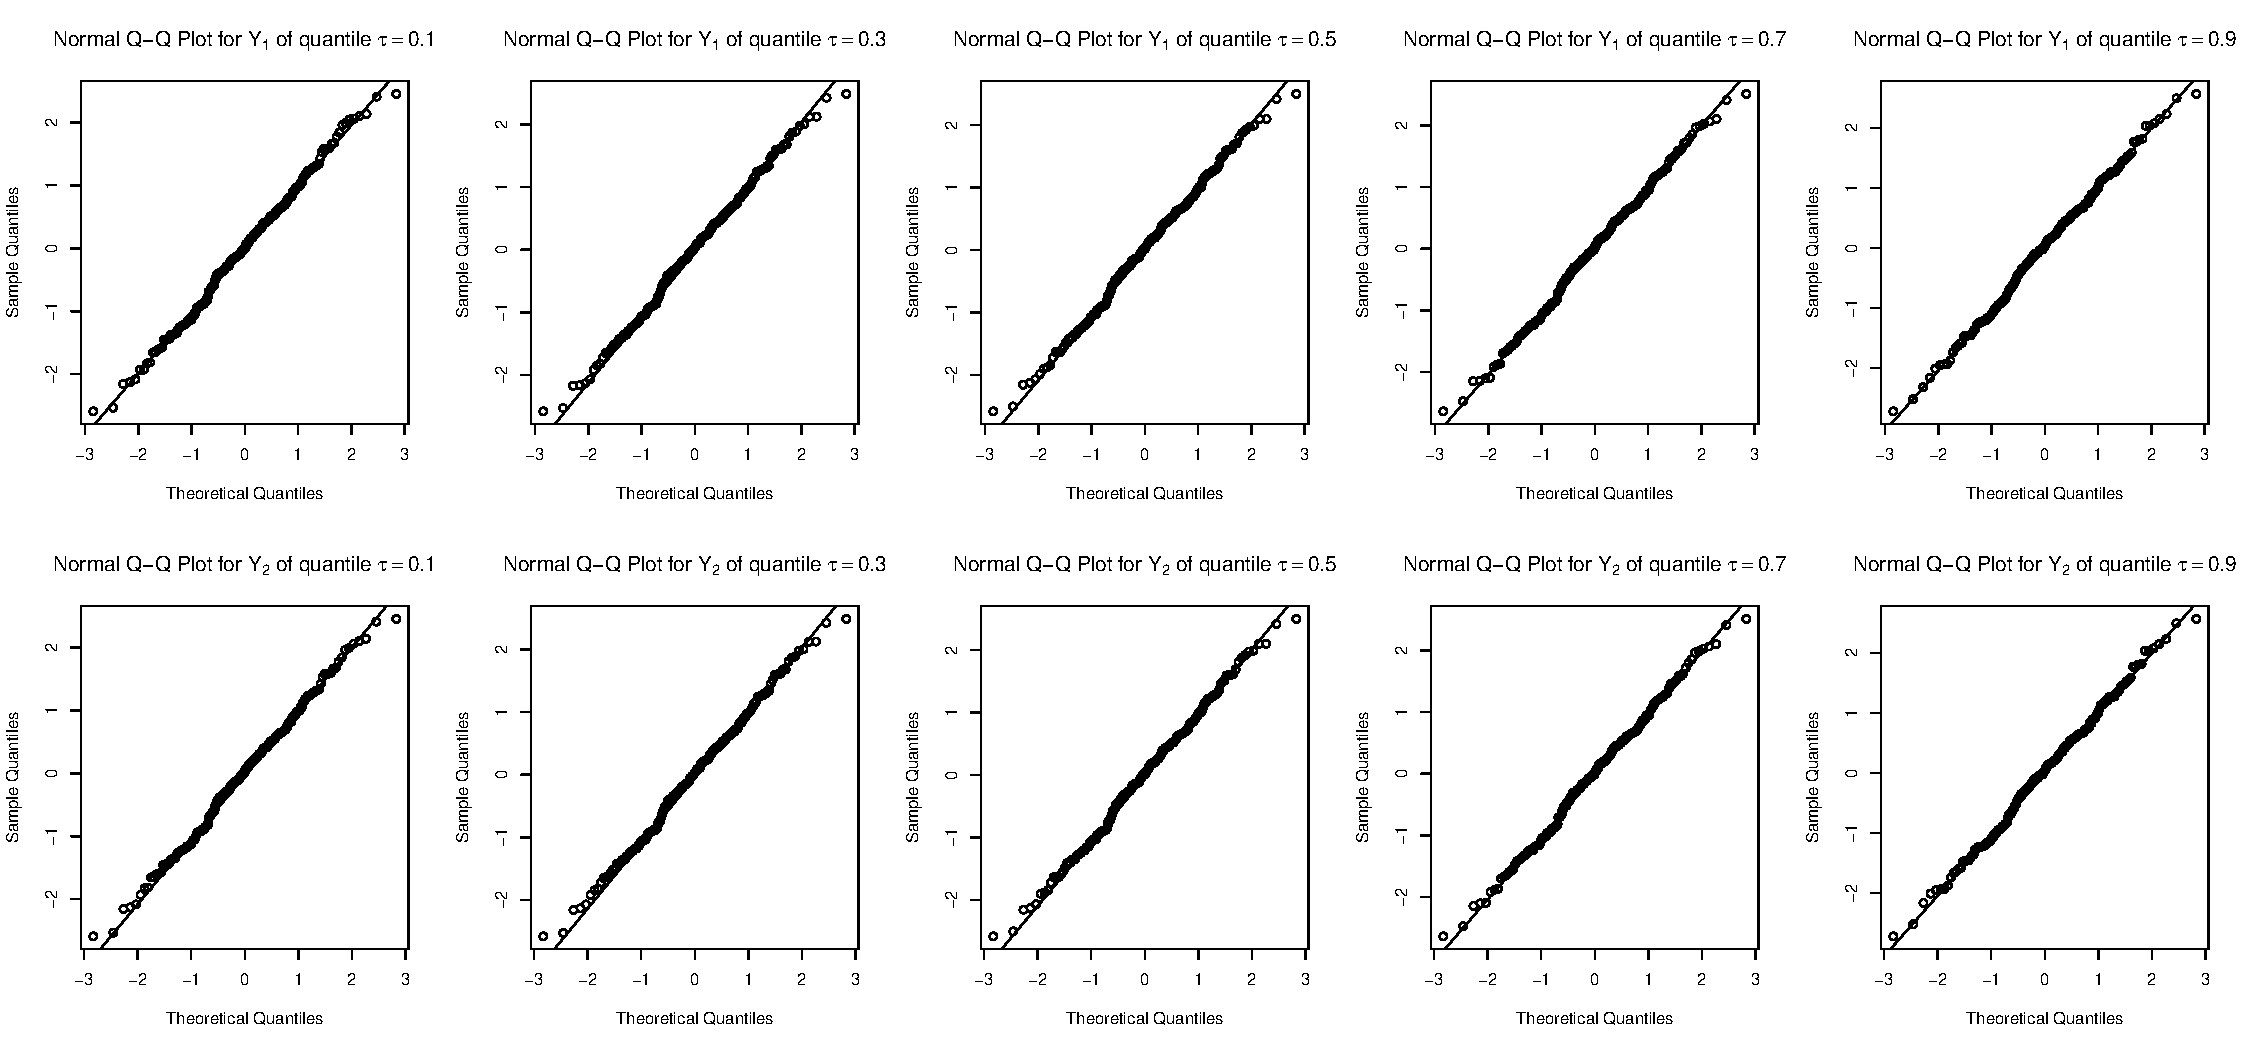
\includegraphics[scale = .4 ]{../image/ToursGoF}}
% \caption{QQ plots for the TOURS data.}
% \label{fig1}
% \end{figure}

\section{Discussion}
\label{ch3:sec:discussion}

In this article, we have developed a marginal quantile regression model
for data with monotone missingness. We use a pattern mixture model to
jointly model the full data response and missingness. Here we estimate
marginal quantile regression coefficients instead of coefficients
conditional on random effects as in \citet{yuan2010}. In addition, our
approach allows non-parallel quantile lines over different quantiles
via the mixture distribution and allows for sensitivity analysis which
is essential for the analysis of missing data \citep{nas2010}.

Our method allows the missingness to be non-ignorable.
We illustrated how to find sensitivity parameters to allow different missing data mechanisms.
The recursive integration algorithm simplifies computation and can be easily implemented even in high dimensions.
Simulation studies demonstrate that our approach has smaller MSE than the traditional frequentist method rq function for the missing component.
And it has advantages over BZ for inference on most quantile regressions even when the tails of the distribution are non-standard (e.g., heavy tails and skewness) since we assume a
multivariate mixture of normals distribution for each component in the pattern mixture model.
We can also conduct inference using a Bayesian non-parametric model, for example, a Dirichlet process mixture which would not require choosing the number of components in the mixture model.
However, efficient computational algorithms would need to be developed for those settings;  we are currently working on this.
Our current approach is implemented with the R package ``qrmissing'' which can be downloaded from the first author's website: \url{https://github.com/liuminzhao/qrmissing}.

\section*{Acknowledgments}

This study is partially supported by NIH grants CA85295 and CA183854.

\bibliographystyle{biom}
\bibliography{qr-missing-reference}

\end{document}

%%% Local Variables:
%%% mode: latex
%%% TeX-master: t
%%% End:
